\documentclass[11pt]{article}
\usepackage{amsmath}
\usepackage{graphicx,epsf}
\usepackage{tabularx,amsmath,amssymb}
\usepackage{float,epsfig,multirow,rotating,times}
%\usepackage{wrapfig}
\usepackage{enumerate}
\usepackage{hyperref}
%\usepackage{natbib}
%\usepackage[dvips, dviwin]{graphics,graphicx}
\usepackage{graphics,graphicx}
\usepackage{color}
\usepackage{pdfpages}
\usepackage{subfigure}
%\usepackage{movie15}
%\usepackage{animate}
%\usepackage{graphicx}
%\DeclareGraphicsExtensions{.gif, .ps, .eps, .png,.pdf}
%\DeclareGraphicsRule{.gif}{png}{}{`convert #1 'png:-'}

%\usepackage[dvips]{color}
%\usepackage{hyperref}
%\textheight 9.5 in
%\textwidth 6.0 in
%\textheight 9.6 in \textwidth 6.5 in \topmargin -1.8cm
%\textheight 9.3 in \textwidth 6.5 in \topmargin -1.5cm
%\oddsidemargin -0.25cm \setlength{\footskip}{1 cm}
%\setlength{\parindent}{0pt}

\newcommand {\ctn}{\citet}
\newcommand {\ctp}{\citep}



\renewcommand{\t}{\ensuremath{\theta}}
\newcommand{\s}{\sigma}
\renewcommand{\a}{\ensuremath{\alpha}}
\renewcommand{\b}{\ensuremath{\beta}}
\newcommand{\g}{\ensuremath{\gamma}}
\renewcommand{\d}{\ensuremath{\delta}}
\newcommand{\e}{\ensuremath{\epsilon}}
\newcommand{\from}{\ensuremath{\leftarrow}}
\newcommand{\bm}{\mathbf}
\renewcommand{\l}{\lambda}
\newcommand {\bzero}{\mbox{\boldmath $0$}}
\newcommand {\bmu}{\mbox{\boldmath $\mu$}}
\newcommand {\bSigma}{\mbox{\boldmath $\Sigma$}}
\newcommand{\dint}{\int\displaylimits}
\newcommand{\boldm}{\mathbf m}
\newcommand{\bL}{\mathbf L}
\newcommand{\bM}{\mathbf M}
\newcommand{\bB}{\mathbf B}
\newcommand{\bC}{\mathbf C}
\newcommand{\bp}{\mathbf p}
\newcommand{\bv}{\mathbf v}
\newcommand{\bx}{\mathbf x}
\newcommand{\by}{\mathbf y}
\newcommand{\bz}{\mathbf z}
\newcommand{\be}{\pmb\e}


\newcommand{\statesp}{\ensuremath{\mathcal X}}
\newcommand{\Y}{\ensuremath{\mathcal Y}}
\newcommand{\D}{\ensuremath{\mathcal D}}
\newcommand{\union}{\cup}
\newcommand{\intersect}{\cap}
\newcommand{\imply}{\Longrightarrow}
\newcommand{\R}{\ensuremath{\mathbb R}}
\newcommand{\E}{\mathrm{E}}

\newcommand{\supr}[2]{{#1}^{(#2)}}
\newcolumntype{Z}{>{\centering\arraybackslash}X}%

\addtolength{\oddsidemargin}{-.75in}%
\addtolength{\evensidemargin}{-.75in}%
\addtolength{\textwidth}{1.5in}%
\addtolength{\textheight}{1.3in}%
\addtolength{\topmargin}{-.8in}%
\linespread{1}

\newtheorem{theorem}{Theorem}
 
\begin{document}

\section{Algorithm}

Our primary interest in this paper lies in simulating from $d$-dimensional target densities $\pi(x_{d})$, comprising of iid target densities $f_{d}(.)$ that are complicated and potentially multimodal (for instance, mixture of normal components) in nature. The main problem in using MCMC for target densities of this form is that the MCMC chain may get stuck in one component for a long period of time. This results in poor exploration of the entire state space and gives biased samples. There has been a lot of research in the MCMC literature that focuses on solving this problem. Two very popular approaches are parallel tempering and simulated tempering. Atchade et al (2010) \cite{Atchade2010} proposed a Metropolis-coupled Markov Cahin algorithm ($MC^3$) and compared the $ESJD$ for the $MC^3$ algorithm with that of the Simulated tempering algorithm. In this paper, we are presenting a modification of the $MC^3$ algorithm by randomizing the inverse temperature spacings for the tempered distributions that are run in parallel. 

We define a sequence of heated or tempered density functions (non-normalized) as ${f_{d}}^{\b_j}(x) = (f_{d}(x))^{\b_j}$ with $0 \leq \b_n < \b_{n-1} \leq < \cdots < \b_{1} < \b_{0}=1$. these $\b_{j}$ are also called inverse temperatures. We propose two algorithms - in one (called $RMC^3$) we run parallely Metropolis-Hastings chains for each ${f_{d}}^{\b_j}$ and for the other (called $RTMC^3$), we run parallely Additive TMCMC chains (refer to Dutta and Bhattacharya (2013) \cite{Dutta2013}, Dey and Bhattacharya (2013) \cite{Dey2013} and Dey and Bhattacharya (2013) \cite{Dey2013b}) for each ${f_{d}}^{\b_j}(.)$. Note that in either method, the chain corresponding to $\b_0$ is the cold chain and the main chain of interest as it corresponds to the original non-tempered density. The main hope behind using these heated or tempered chains for varying $\b_j$ is that chains with smaller inverse temperatures will be able to mix more easily as they would be flatter. We keep a swapping phase in our algorithm, in which we swap the iterates for chains of different inverse temperatures with the hope that they would add some valuable mixing information to the original cold chain corresponding to $b_0$. 

There are two phases wo the $RMC^3$ or the $RTMC^3$ algorithms and these two phases are analogous to the ones recommended by Atchade et al (2010) \cite{Atchade2010}. 

\begin{itemize}
\item Normal iteration step
\item Temperature Swap step
\end{itemize}

In the \textbf{first step}, we update each of the chains (corresponding to each $\b_j$ or inverse temperature) separately either by the RWMH (Random Walk Metropolis Hastings) or by the Additive TMCMC updates in $RMC^3$ and $RTMC^3$ respectively. These parallel chains have target densities ${f_{d}}^{\b_j} (.)$. \\

In the \textbf{second step}, we swap the iterates corresponding to two inverse temperatures. We choose two inverse temperatures $\b_j$ and $\b_k$ and try to swap the iterates $x_j$ and $x_k$ corresponding to ${f_{d}}^{\b_j} (.)$ and ${f_{d}}^{\b_k} (.)$ respectively. We accept the swap with the probability given by 

\newcommand{\fjxj}{{f_d}^{\beta_{j}}(x_j)}
\newcommand{\fjxk}{{f_d}^{\beta_{j}}(x_k)}
\newcommand{\fkxj}{{f_d}^{\beta_{k}}(x_j)}
\newcommand{\fkxk}{{f_d}^{\beta_{k}}(x_k)}

\[ Prob(accepting \; swap)= min \left (1, \frac{\fjxk \fkxj}{\fjxj \fkxk} \right ) \]

Otherwise, the chains remain unchanged. \\

The main question of interest is that how should we choose the inverse temperatures optimally, or rather, if we want to swap the chain with inverse temperature $\b_j$ with another inverse temperature $\b_k$, how should we choose these values optimally. Atchade et al (2010) \cite{Atchade2010} consider the case where we pick adjacent inverse temperatures for swapping at a specific distance, say $\b$ and $\b+\e$ and our main query of interest then is how to optimally choose $\e$. We propose here an alternative where this $\e$ is random and has a distribution on the positive support, for convenience, we consider the case that $\e \sim TN_{>0}(0, \frac{l^2}{d})$ for dimension $d$ and our new focus would be to choose an appropriate scaling $l$. Note that if $l$ is large, then $\e$ would tend to be larger and this would result in greater rejection of the swaps. Again, if $l$ is small, then we shall have higher acceptance of swaps but the two swapping inverse temperatures would be very close to each other and so, ideally, with the swapping iterates also likely to be close, thereby resulting in poor mixing.  So, in the next section, we shall deal with the problem of determining the optimal value of the scaling $l$. We shall show that while in Atchade et al's paper \cite{Atchade2010}, their choice of $\e$ leads to an optimal acceptance rate of $0.234$, our method corresponding to the optimal scaling $l_{opt}$ gives an optimal acceptance rate of $0.439$ which is almost double that of the $MC^3$ algorithm. Note that while in the $MC^3$ algorithm, the inverse temperatures are equally spaced, in our proposed methods ($RMC^3$ or $RTMC^3$) the inverse temperatures are irregularly spaced due to the inherent randomness in $\e$ and that lends extra flexibility to our algorithm. 



\begin{theorem}
Consider the $RMC^3$ or the $RTMC^3$ chain with a target density $\pi$ and allow swap of the temperatures between two consecutive inverse temperature heated chains only, namely $\b$ and $\b+\l$ where we consider $\l$ to have the distribution $TN_{>0} (0, \frac{l^2}{d})$. Then as the dimension of the chain $d \rightarrow \infty$, the ESJD is maximized when we choose $l$ to be maximize the function 
$D(l)= \int_{Z} {l^2 Z^2 \Phi \left (-\frac{l|Z|\eta(\b)}{\sqrt{2}} \right ) \phi(Z)} dZ$
and this optimal choice of $l$ can be shown to lead to a limiting expected acceptance rate of $0.439$ which is almost twice that of the standard $MC^3$ algorithm. 
\end{theorem}


\section{Proof of the main theorem}

We consider the specific problem of determining the optimal temperatures of the sequence of the heated chains in the Randomized Metropolis Coupled MCMC ($RMC^3$) and Randomized Additive Transformation based MCMC ($RTMC^3$). Suppose we are at the $n$ th iteration and we denote the filtration, or the $\sigma$-field formed by the iterates upto the $n-1$ iterations over all the parallely run chains to be $\mathcal{F}_{n-1}$. We consider the swapping between the temperatures $\beta$ and $\beta+Y$ where we assume that $Y \sim TN_{>0}(0,\frac{l^2}{d})$ where $TN_{>0} ()$ represents the truncated normal random variable left truncated at $0$. We assume that $\beta > 0$, $\l$ is a random variable that $\l >0$ with probability $1$ and $\beta + \l \leq 1$ with probability $1$ as $d \rightarrow \infty$ for $\beta \in (0,1)$. We wish to find the optimal vale of $l$ under the assumption of stationarity of the chain ($X \sim \prod_{j=1}^{n} {f_{d}}^{\beta_j}$) Let us define $\beta^{\star}  =\beta+\l$ if we accept the swap and $\beta^{\star}=\beta$ otherwise. If the proposed step is accepted, then we move to the new point $\beta^{\star}$ and if it is rejected, then we stay where we are at $\beta$.The general approach that we follow for finding out an optimal choice of $l$ would be to maximize the stationary expected squared jumping distance (ESJD) as 

%\newcommand{\fjxj}{{f_d}^{\beta_{j}}(x_j)}
%\newcommand{\fjxk}{{f_d}^{\beta_{j}}(x_k)}
%\newcommand{\fkxj}{{f_d}^{\beta_{k}}(x_j)}
%\newcommand{\fkxk}{{f_d}^{\beta_{k}}(x_k)}

\begin{align*}
ESJD & =  E_{\pi} (\beta^{\star} - \beta)^2  \\
	 & =  \int { \l^2 E_{\pi} \left [ min \left (1, \frac{\fjxk \fkxj}{\fjxj \fkxk} \right ) \right ]} \\
\end{align*} 

where $x_j$ is the present iterate of the chain corresponding to the $j$th heated chain denoted by the suffix $\beta_{j}$ and $x_{k}$ is the present iterate corresponding to the $k$th heated chain. Consider the target density to be $\pi_{d}(x) = \prod_{i=1}^{d} f(x_{i})$ and the heated chain with suffix $\beta$ is given by $ {\pi_{d}}^{\beta} (x) = \prod_{i=1}^{d} f(x_{i})^{\beta}$. Note that we can write $Y=\frac{lZ}{\sqrt{d}}$ where $Z$ is $TN_{>0}(0,1)$ random variable. We shall show that for both the $RMC^{3}$ and the $RTMC^{3}$ algorithms, as $d \rightarrow \infty$, the ESJD is maximized when $l$ is chosen to maximize $2\int {l^2 z^2 \Phi(-\frac{lz\sqrt{I(\beta)}}{2})}$. This is equivalent to finding out the optimal scaling for the Additive TMCMC approach with the same target density. The acceptance probability given the random variable $\l$ is given by $\alpha(\l) = min (1, exp(B))$ where $B$ is given by

\newcommand{\fby}{{f_d}^{\beta}(y)}
\newcommand{\fbex}{{f_d}^{\beta+\l}(x)}
\newcommand{\fbx}{{f_d}^{\beta}(x)}
\newcommand{\fbey}{{f_d}^{\beta+\l}(y)}

\[ B = ln \left (\frac{\fby \fbex}{\fbx \fbey} \right )     \]

This can be reduced to the expression
\begin{align*}
 B & = \left (ln(\fby) -ln(\fbey) \right) - \left (ln(\fbx) - ln(\fbex) \right) \\
	 & = R_{d}(y) -R_{d}(x)  \\
	 \end{align*}



Let us denote $h(x)=ln(f(x))$ and we know that $\fbx= \prod_{i=1}^{d} {f(x_i)^{\beta}}$. Using this, the above expression reduces to the following

\[ R_{d}(x)= \beta \sum_{i=1}^{d} g(x_{i}) -(\b+\l) \sum_{i=1}^{d} g(x_{i}) = -\sum_{i=1}^{d} \frac{lZ}{\sqrt{d}} g(x_{i}) \]

Now we consider the expectation and the variance of the function $g$ under the density function $f^{\beta}$, suitably normalized. Then the expectation and the variance of the function $g$ with respect to the normalized density measure $f^{\b}$ is given by 

\[  E^{\b} (g) = \frac{\int log(f(x)) f^{\b}(x)dx}{\int f^{\b}(dx)} = m(\b)  \]

\[  V^{\b}(g) =  \frac{\int (log f(x))^2 f^{\b}(x)dx}{\int f^{\b}(x)dx} - (E^{\b}(g))^2 = \eta^2 (\b) \]

Then the conditional expectation and the conditional variance of $R_d$ given the random variable $Z$ is given by

\[ E^{\beta} (R_{d}(x)|Z) = -\sqrt{d}lZ E^{\b} (g) = \mu_{\b,Z}  \]

\[ V^{\b} (R_{d}(x) |Z) = d l^{2} Z^{2} V^{\b} (g) = \sigma^2_{\beta,Z}  \]

where the expressions for $E^{\b}(g)$ and $V^{\b}(g)$ are given above. It can be shown by differentiating $\mu_{b,Z} $ with respect to $\b$ that 

\[ m^{'}(\b) = \eta^{2} (\b)   \hspace{2 cm}   \mu^{'}_{b,Z} = -\frac{\sqrt{d}}{lZ} \sigma^2_{\b,Z}    \]

This implies that 

\[ R_{d}(y) - R_{d}(x) = -\frac{lZ}{\sqrt{d}} \sum_{i=1}^{d} (g(y_{i})-g(x_{i}))  \]

Our aim is to derive the asymptotic distribution of the quantity $R_{d}(y)-R_{d}(x)$ and the characteristic function is given by 

\begin{align*}
\phi_{d}(t |Z, \mathcal{F}_{n-1})  & = E |_{Z,  \mathcal{F}_{n-1}} \left [exp\phantom{\frac{1}{2}} \left ( \phantom{\frac{1}{2}} it(R_{d}(y)-R_{d}(x)) \right) \right ]  \\
  & = E |_{Z,  \mathcal{F}_{n-1}} \left [ exp \left (-it \frac{lZ}{\sqrt{d}} \sum_{i=1}^{d} (g(y_{i}) -g(x_{i}))\right ) \right ]  \\
  & = E _{Y|{Z,  \mathcal{F}_{n-1}}}\left [ exp \left (-it \frac{lZ}{\sqrt{d}} \sum_{i=1}^{d} \{g(y_i) - m(\b+\e) \} \right )  \right ]  E_{X|{Z,  \mathcal{F}_{n-1}}} \left [ exp( \left (it \frac{lZ}{\sqrt{d}} \sum_{i=1}^{d} \{g(x_i) - m(\b)\} \right )  \right ] \\
  & \qquad \qquad \times E |_{{Z},  \mathcal{F}_{n-1}} \left [ exp \left (-it \frac{lZ}{\sqrt{d}}(m(\b+\e) - m(\b)) \right ) \right ] \\
\end{align*}

where $\mathcal{F}_{n-1}$ is the filtration generated by the $n-1$ iterations of all the parallel chains in the $RMC^{3}$ or the $RTMC^{3}$ algorithm corresponding to all the inverse temperatures (meaning all the heated chains with various degrees of heating) along with the cold chain- the main chain of interest.


By the application of the Central Limit theorem we know that $\frac{1}{\sqrt{d}} \sum_{i=1}^{d} (g(x_{i})- m(\b))  \sim N(0, \eta^{2}(\b)) $ where $\textbf{x} \sim {f_d}^{\beta}$. This implies by the Taylor series theorem that 

\begin{equation} \label{eq:eqYZ}
E_{Y|Z} \left [ exp(-it \frac{lZ}{\sqrt{d}}) \sum_{i=1}^{d} {g(y_i) - m(\b+\l) } \right ] = 1-\frac{l^2 Z^2}{2d} \eta^2(\b+Y)+o \left (\frac{1}{d} \right) 
\end{equation}

%
%\begin{align*}
%\E_{Z} E_{Y|Z} \left [ exp(-it \frac{lZ}{\sqrt{d}}) \sum_{i=1}^{d} {g(y_i) - m(\b+\e) } \right ] & = & \int \left \{ 1-\frac{l^2 Z^2}{2d} \eta^2(\b+Y)+o \left (\frac{1}{d} \right) \right \} \phi(Z) dZ  \\
%& = & 1- \int \frac{l^2 Z^2}{2d} \eta^2 \left (\b+ \frac{lZ}{\sqrt{d}} \right) \phi(Z)dZ +o \left (\frac{1}{d} \right) \\
%& = & 1 - \int \frac{l^2 Z^2}{2d} \eta^2(\b)\phi(Z)dZ + o \left(\frac{1}{d} \right)  
%\end{align*}


\begin{equation}
\label{eq:eqXZ}
E_{X|Z} \left [ exp(-it \frac{lZ}{\sqrt{d}}) \sum_{i=1}^{d} {g(x_i) - m(\b) } \right ] = 1-\frac{l^2 Z^2}{2d} \eta^2(\b)+o \left (\frac{1}{d} \right)
\end{equation}

%
%\begin{align*}
%\E_{Z} E_{X|Z} \left [ exp(-it \frac{lZ}{\sqrt{d}}) \sum_{i=1}^{d} {g(x_i) - m(\b) } \right ] & = & \int \left \{ 1-\frac{l^2 Z^2}{2d} \eta^2(\b)+o \left (\frac{1}{d} \right) \right \} \phi(Z) dZ   \\
%& = & 1- \int \frac{l^2 Z^2}{2d} \eta^2(\b) \phi(Z)dZ +o \left (\frac{1}{d} \right) \\
%\end{align*}

Also we have given $Z$,
\begin{equation} \label{eq:eqZ}
itlZ \sqrt{d} (m(\b+Y) -m(\b)) \rightarrow  it l^2 Z^2 \eta^2 (\b)   \hspace{1 cm} as \; d \rightarrow \infty
\end{equation}


This  follows from the fact that given $Z$, the variable $Y$ is known and then from the definition

\[ \underset{d \rightarrow \infty} {Lt} \frac{m(\b+Y) - m(\b)}{Y}  \rightarrow m^{'}(\b) = \eta^{2}(\b)  \]


So from the above equations \textbf{Eq~\ref{eq:eqYZ}}, \textbf{Eq~\ref{eq:eqXZ}} and \textbf{Eq~\ref{eq:eqZ}},  it follows that $\phi_{d}(t |Z, \mathcal{F}_{n-1})$ converges to 
$$\phi^{\star}(t|Z,\mathcal{F}_{n-1})= exp(-itl^2 \eta^2(\b) Z^2 - l^2 t^2 Z^2  \eta^2(\b) )$$. 


This is the characteristic function of $ N(-l^2 \eta^2(\b) Z^2, l^2 t^2 Z^2\eta^2(\b) )$ density given the random variable $Z$. 

Note that a standard result (see Roberts et al. 1997 \cite{Roberts1997}, Dey and Bhattacharya \cite{Dey2013}) that for a random variable $X \sim N(\mu, \sigma^2)$ 

\[ E \left ( \vphantom{\frac{1}{2}} min (1, exp(X)) \right) = \Phi(\frac{\mu}{\s}) + exp(\mu + \frac{\s}{2}) \Phi(-\s - \frac{\mu}{\s})    \]


From the above calculations, we have shown that the limiting distribution of $B \sim N(-l^2 \eta^2(\b) Z^2, l^2 t^2 Z^2\eta^2(\b) )$ and hence, the limiting expected acceptance rate of the swap given $\l$ or equivalently given $Z$ is given by 

\[ E|_{Z, \mathcal{F}_{n-1}} \left (min (1, exp(B(Z))) \right )  \approx 2 \Phi(-\frac{lZ \eta(\b)}{\sqrt{2}})  \]

However, as per our assumption the heatings are not uniformly distributed as in the standard $MC^{3}$ and the randomness is expressed in terms of $Z$ which has a $TN_{>0} (0,1)$ distribution. Under this set up, we have 


\[ ESJD = \int_{Z>0} { \frac{l^2 Z^2}{d}  E_{Z,\mathcal{F}_{n-1}} \left ( \phantom{\frac{1}{2}} min \left (1,exp(B(Z)) \right) \right ) \phi^{+}(Z) dZ }  \]

Then in the limit we can write this as 

\begin{equation}\label{eq:esjd1}
ESJD \approx 2 \int_{Z>0}  {\frac{l^2 Z^2}{d} \Phi \left (-\frac{lZ \eta(\b)}{\sqrt{2}} \right ) \phi^{+}(Z) dZ }
\end{equation}

where $\phi^{+} (.)$ is the density function for the $TN_{>0} (.)$ random variable. Note that instead of generating a $Z$ from $TN_{>0}(0,1)$ random variable and updating $\beta$ by $\b + \frac{lZ}{\sqrt{d}}$, we can equivalently generate $Z$ from $N(0,1)$ distribution and then update $\b$ by $\b + \frac{l|Z|}{\sqrt{d}}$. Using this analogy, it trivially follows from \textbf{Eqn~\ref{eq:esjd1}} that

\begin{equation}
ESJD \approx 4 \int_{Z}  {\frac{l^2 Z^2}{d} \Phi \left (-\frac{l|Z| \eta(\b)}{\sqrt{2}} \right ) \phi(Z) dZ }
\end{equation}

In order to maximize the $ESJD$ with respect to $l$ we aim to optimize the function 

\[ \mathcal{D}(l) = \int_{Z} {l^2 Z^2 \Phi \left (-\frac{l|Z| \eta(\b)}{\sqrt{2}} \right ) \phi(Z)} dZ \]


with respect to $l$. This is analogous to the expression for the diffusion speed we obtained in Dey and Bhattacharya (2013)  \cite{Dey2013}. As has been shown in that paper already, the maxima of this function is attained at the value of $l$ 

\[  l_{opt} = \frac{2.426}{\eta(\b)} \]

and the value of the optimal acceptance rate corresponding to this optimal value of $l$ is given by 

\[ \alpha_{opt} = 4 \int_{Z} \Phi \left (-\frac{l_{opt}|Z|\eta(\b)}{\sqrt{2}} \right) \phi(Z) dZ  \approx 0.439 \]


This optimal value of the acceptance rate is higher than that of the $MC^{3}$ algorithm derived in Atchade et al. (2010) \cite{Atchade2010}. We emphasize the fact that under the optimal scaling for our proposed algorithm, we have higher limiting expected acceptance rate of the swaps, meaning higher degree of exchange between the parallel chains and this will lead to better exploration of the state space. Also the graphs of $\mathcal{D}(l)$ implies that the $ESJD$ for both the $MC^3$ and that of $RMC^3$ / $RTMC^3$ are close corresponding to $l_{opt}$ but that of $MC^{3}$ is slightly higher and for higher values of $l$, the $ESJD$ for the $MC^3$ chain falls rapidly while that of the $RMC^3$ or $RTMC^3$ chains remain more or less stable for a wide range of $l$. 

Note that one big assumption in this calculation is that the process is in stationarity. The higher value of $D(l_{opt})$ in $MC^3$ implies that the ESJD would be marginally higher under stationarity compared to that of $RMC^3$ or $RTMC^3$ algorithms for the optimal scaling. But to have a valid comparison of the two methods, we must compare the performance even under non-stationarity, and under non-stationarity, our algorithm has a clear edge over $MC^3$ because it has higher acceptance rate of the swaps and hence has better exploration of the state space compared to the $MC^3$. 

\begin{figure}  \centering 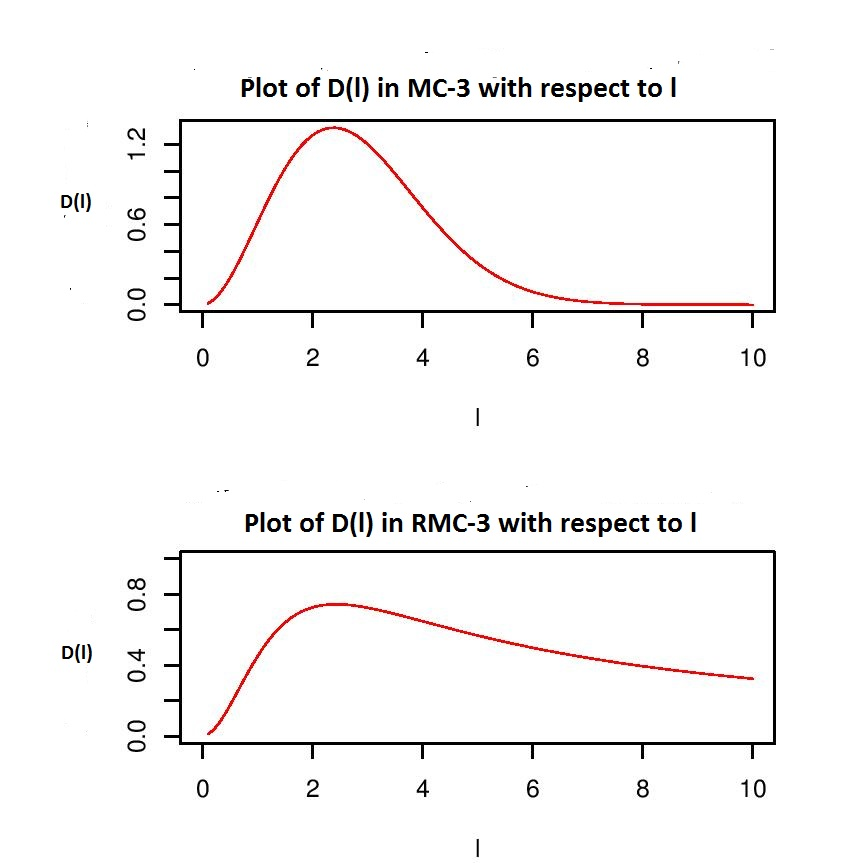
\includegraphics[width=15cm,keepaspectratio]{diffspeed}  
\caption{The plots of $D(l)$ which is proportional to the $ESJD$ with respect to $l$ for the $MC^3$ and the $RMC^3$ algorithms.} \label{fig:fig4} \end{figure}




\begin{thebibliography}{widestlabel}
\bibitem{Roberts1997} Roberts, G.O., Gelman, A. and Gilks, W.R. (1997), "Weak convergence and Optimal Scaling of Random Walk Metropolis algorithms" \emph{Ann.Appl.Prob}, 7, 110-120 
\bibitem{Dey2013} Dey K.K. and Bhattacharya S.(2013), "On Optimal Scaling of Additive Transformation Based Markov Chain Monte Carlo", \emph{preprint}, arxiv:1307.1446
\bibitem{Atchade2010} Atchade, Y.F., Roberts, G.O. and Rosenthal, J.S. (2010), "Towards Optimal Scaling of Metropolis-coupled Markoc Chain Monte Carlo" \emph{Stat Comput}, 21, 555-568 
\bibitem{Dutta2013} Dutta, S. and Bhattacharya, S. (2013), "Markov Chain Monte Carlo Based on Deterministic Transformations" \emph{Stat Methodology}, 16, 100-116
\bibitem{Dey2013b} Dey, K.K. and Bhattacharya, S. (2013), "On Geometric Ergodicity of Additive and Multiplicative Transformation Based Markov Chain Monte Carlo in High Dimensions", \emph{preprint}, arXiv:1312.0915 
\end{thebibliography}
\end{document}






